%\documentclass{beamer}
\documentclass[t]{beamer} 	%to produce printable hand-outs
% user packages
\usepackage{amssymb}
\usepackage{graphicx} % Allows including images
\usepackage{booktabs} % Allows the use of \toprule, \midrule and \bottomrule in tables
\usepackage[export]{adjustbox}[2011/08/13]
\usepackage{listings}
\usepackage{makeidx}
\usepackage{amsmath}
\usepackage[natbibapa]{apacite}
\usepackage{acro}
\usepackage{subcaption}
\usepackage[export]{adjustbox}
\usepackage{framed}
\usepackage{makecell}
\usepackage{chngpage}
\usepackage{float}
\usepackage{setspace}
\usepackage{mfirstuc}
\usepackage{url}
\usepackage[ruled,vlined,linesnumbered]{algorithm2e}
\usepackage[symbols,nogroupskip,sort=none]{glossaries-extra}
\usepackage{animate}
\usepackage[most]{tcolorbox}

%load theme
\usetheme{usyd2016}

\addtobeamertemplate{navigation symbols}{}{%
    \usebeamerfont{footline}%
    \usebeamercolor[fg]{footline}%
    \hspace{1em}%
    \insertframenumber/\inserttotalframenumber
}

\AtBeginSection{\frame{\sectionpage}}

\newtcolorbox[auto counter]{pabox}[1]{%
    colback=white,
    colframe=structure.fg,
    colbacktitle=white!90!structure.fg,
    coltitle=black,
    fonttitle=\bfseries, 
    enhanced,
	title=#1,
    attach boxed title to top left={yshift=-2mm, xshift=0.5cm}
}

% New commands %
\newcommand{\bi}{\begin{itemize}}
	\newcommand{\ei}{\end{itemize}}
	\newcommand{\be}{\begin{enumerate}}
	\newcommand{\ee}{\end{enumerate}}
	
	\newcommand{\items}{\smallskip\item}
	\newcommand{\itemm}{\medskip\item}
	\newcommand{\itemb}{\bigskip\item}
	
	\newcommand{\half}{\frac{1}{2}}
	\newcommand{\quarter}{\frac{1}{4}}
	\newcommand{\ALPHA}{{\sqrt{1+2\mu\sigma}}/{\sigma}}
	\newcommand{\w}{\sqrt{\mu^2+\alpha^2}-\mu}
	
	\newcommand{\tabularnewline}{\\}
	
	\newcommand{\alphanew}{\frac{\mu(1-\sigma^2)}{\sigma^2}}
	\newcommand{\betanew}{\frac{(1-\mu)(1-\sigma^2)}{\sigma^2}}
	
	
	\renewcommand{\small}{\scriptsize}
	
	%\newcommand{\grb}[1]{\mbox{\boldmath $#1$}}
	\newcommand{\grb}[1]{#1}
	\newcommand{\x}{x}
	\newcommand{\X}{X}
	\newcommand{\given}{|}
	\newcommand{\E}{\mathbb{E}}
	\newcommand{\p}{\partial}
	\newcommand{\Var}{\mathbb{V}}

% use if you want greyed out steps rather than invisible
%\setbeamercovered{transparent}	

\setbeamertemplate{blocks}[rounded][shadow]


%---------------------- Title Slide page setup -----------------------%

% document details
\title{Distributional Regression}
\subtitle{Sydney Informatics Hub Masterclass series} % (optional)
\author{Stanislaus Stadlmann}
\institute{Sydney Informatics Hub}
\date{May 25, 2023} % (optional)

%--------------------------------------------------------------------
%                           Begin Document
%--------------------------------------------------------------------

\begin{document}
	
%--------------------------------------------------------------------
%                           Title Slide
%--------------------------------------------------------------------

\begin{frame}
	\titlepage
\end{frame}

%---------------------- Table of Contents Slide --------------------%

\begin{frame}
	\frametitle{Overview} % Table of contents slide, comment this block out to remove it
	\tableofcontents 
\end{frame}

%---------------------- Section: About SIH masterclasses --------------------%
\section{About SIH masterclasses and this talk}

\begin{frame}{SIH masterclasses}
	\textbf{About}
	\begin{itemize}
		\item Standalone workshops on a particular topic
		\item Third thursday of the month
		\item Check out our "upcoming workshops" on the SIH website
	\end{itemize}
	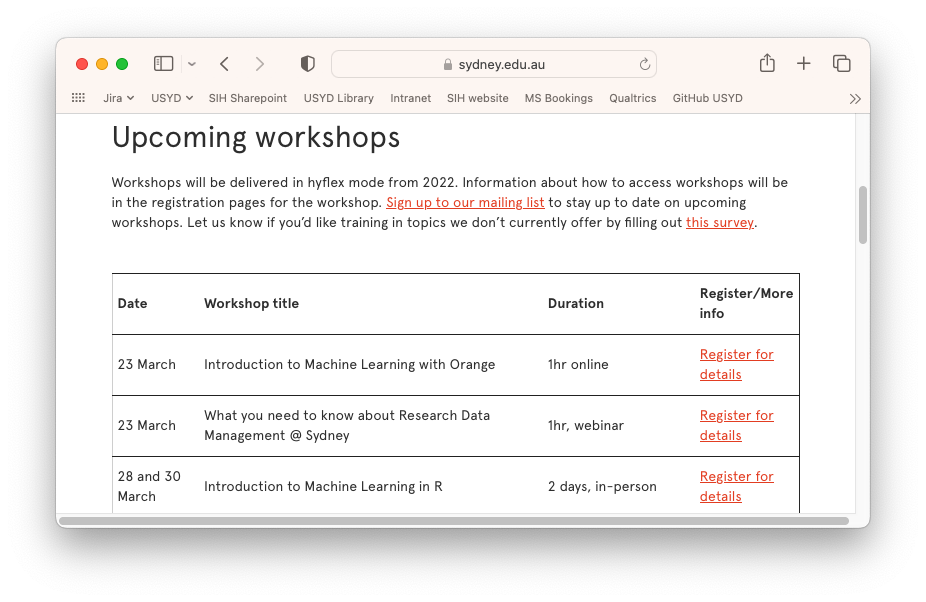
\includegraphics[width=\textwidth]{images/upcoming_workshops.png}
\end{frame}

\begin{frame}{This talk}
	\textbf{More info}
	\begin{itemize}
		\item Gillian Heller's talk at JB Douglas awards 2020
		\item ``The new normal: distributional regression''
		\item Re-written for new audience
		\item Recorded
	\end{itemize}
	\begin{figure}
		\centering
		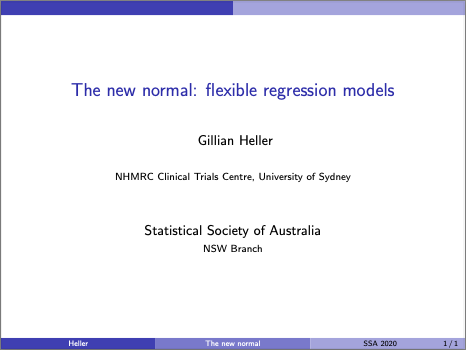
\includegraphics[width=0.6\textwidth]{images/gillian_talk.png}
	\end{figure}
\end{frame}

%---------------------- Section: A brief history of Regression Analysis --------------------%

\section{How did we get here?}

\begin{frame}{Regression Analysis: A brief history}
	\textbf{How long is a metre?}
	\begin{figure}
		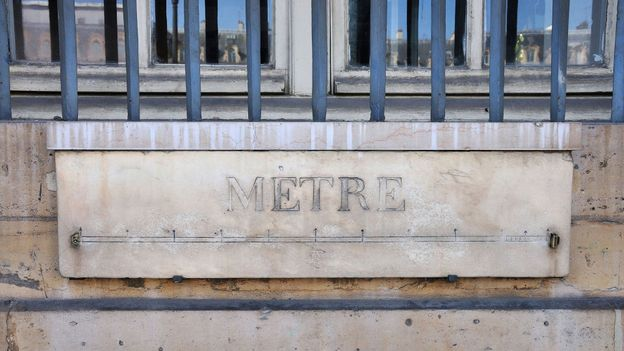
\includegraphics[width=\textwidth]{images/metre.jpg}
		\caption*{The last original metre in Paris, France}
	\end{figure}
\end{frame}

\begin{frame}{Regression Analysis: A brief history}
	\textbf{How long is a metre?}
	\begin{itemize}
		\item 1789: French Revolution
		\item Desire to replace features of the Ancien Régime
		\item The \textit{toise}: "distance between the fingertips of the outstretched arms of a man" \citep{toise}
	\end{itemize}
	\pause
	\begin{pabox}{Definition}
		$m = \frac{d}{10,000,000}$,
		where $d$ is the distance between Equator and North Pole
	\end{pabox}
	\pause
	But: How long is this distance $d$?
\end{frame}

\begin{frame}{Regression Analysis: A brief history}
	\begin{columns}
		\begin{column}[T]{0.5\textwidth}
			\textbf{How long is a metre?}
			\begin{itemize}
				\item A portion of the quadrant to be surveyed within France
				\item Adrien-Marie Legendre tasked to combine multiple measurements
				\item His publication: \citet{legendre1805} comes from that
				\item ``Invention'' of the Least Squares method
				\item Spicy: Gauss later claimed he had already been using this technique since 1775.
			\end{itemize}
		\end{column}
		\begin{column}[T]{0.5\textwidth}
			\centering
			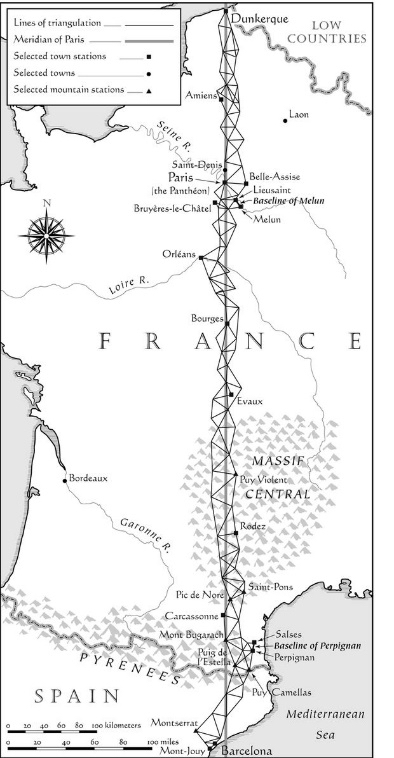
\includegraphics[height = 0.85\textheight]{images/paris_map}
		\end{column}
	\end{columns}

\end{frame}

\begin{frame}{Regression Analysis: A brief history}
	\textbf{Linear Regression Analysis}
	\begin{figure}
		\centering
	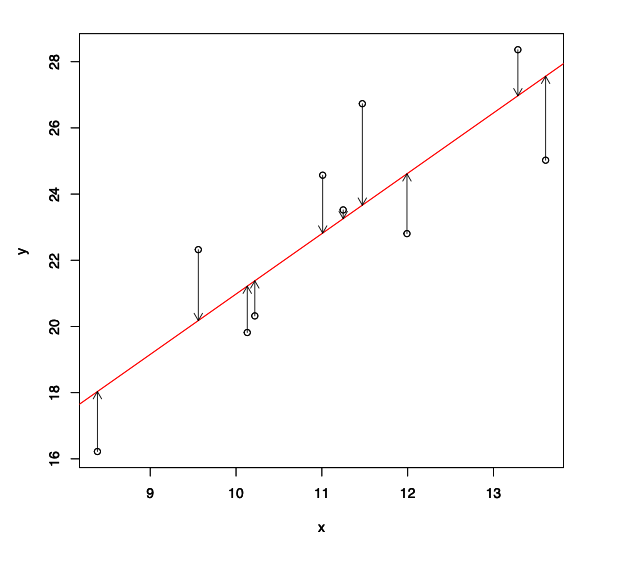
\includegraphics[width=0.85\textwidth]{images/least_squares}
	\end{figure}
\end{frame}

\begin{frame}{Regression Analysis: A brief history}
	\textbf{Linear Regression: Model Assumptions}
	\begin{align*}
		y_i &= x_i^\top\beta+\epsilon_i \\
		\epsilon_i&\stackrel{\hbox{\tiny{ind}}}{\sim} \mathcal{N}(0,\sigma^2)
	\end{align*}
	\begin{itemize}
	\item normality of errors
	\item homoscedasticity of errors: \\
	$\Var(y_i)=\sigma^2$
	\item independence
	\end{itemize}
\end{frame}

\begin{frame}{Regression Analysis: A brief history}
	\textbf{Error distribution} \\
	But what if our errors are not normally distributed? \\
	$\:$
	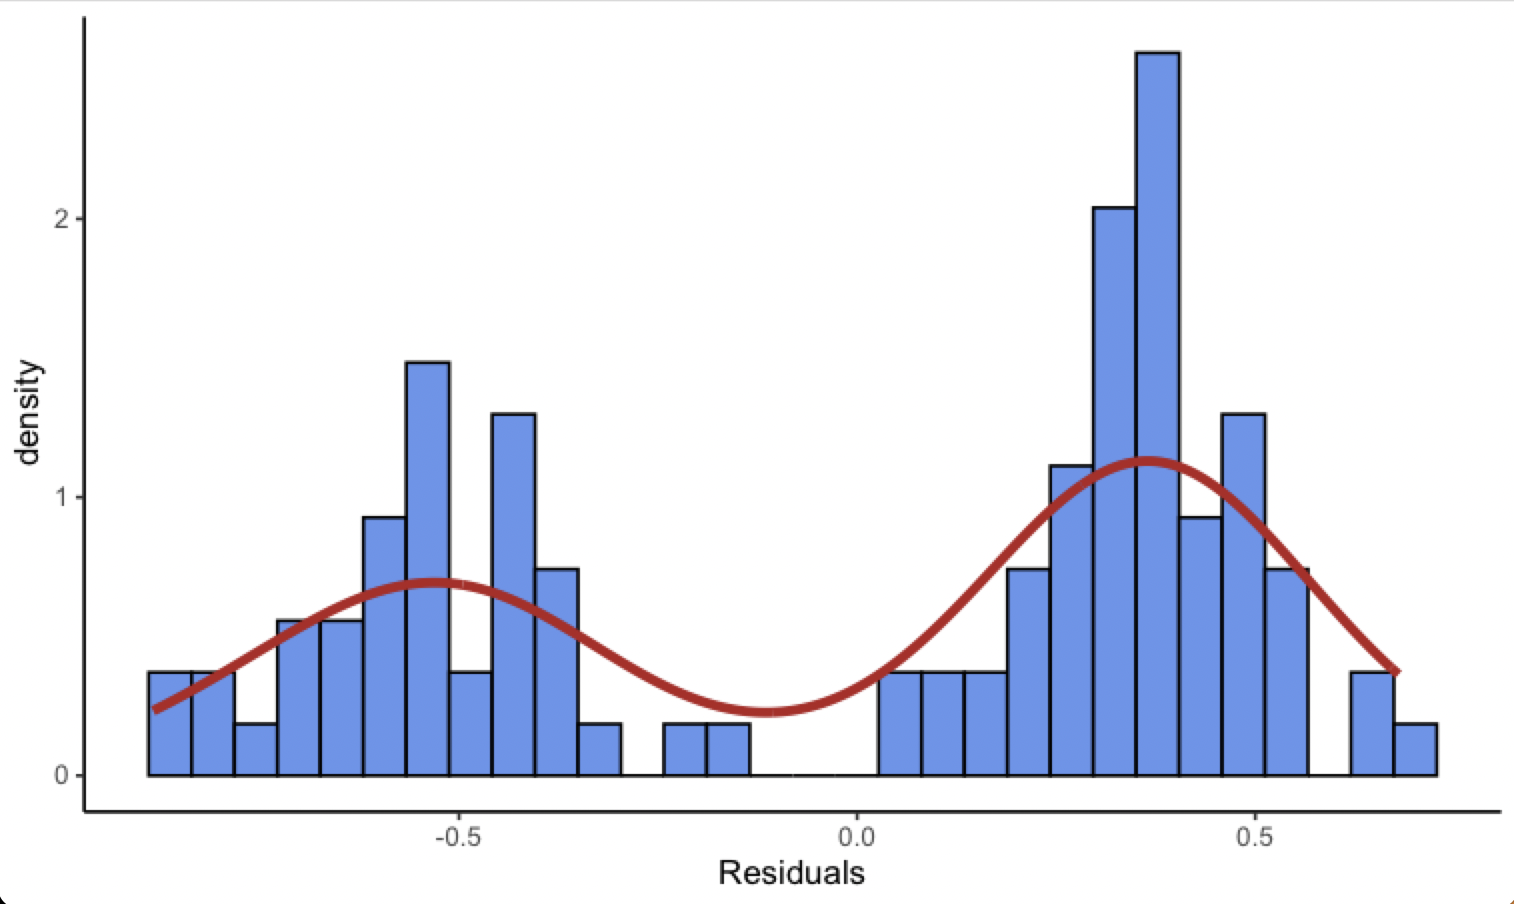
\includegraphics[width=\textwidth, trim={0.2cm 0cm 0.2cm 0.5cm}, clip]{images/residuals.png}
\end{frame}

\begin{frame}{Regression Analysis: A brief history}
	\textbf{Generalized Linear Models} \\
	``Theoretical and applied statistics were both convulsed by the publication of the GLM paper
		by Nelder and Wedderburn (1972)." \citep{murray2018}
	\begin{figure}
		\centering
		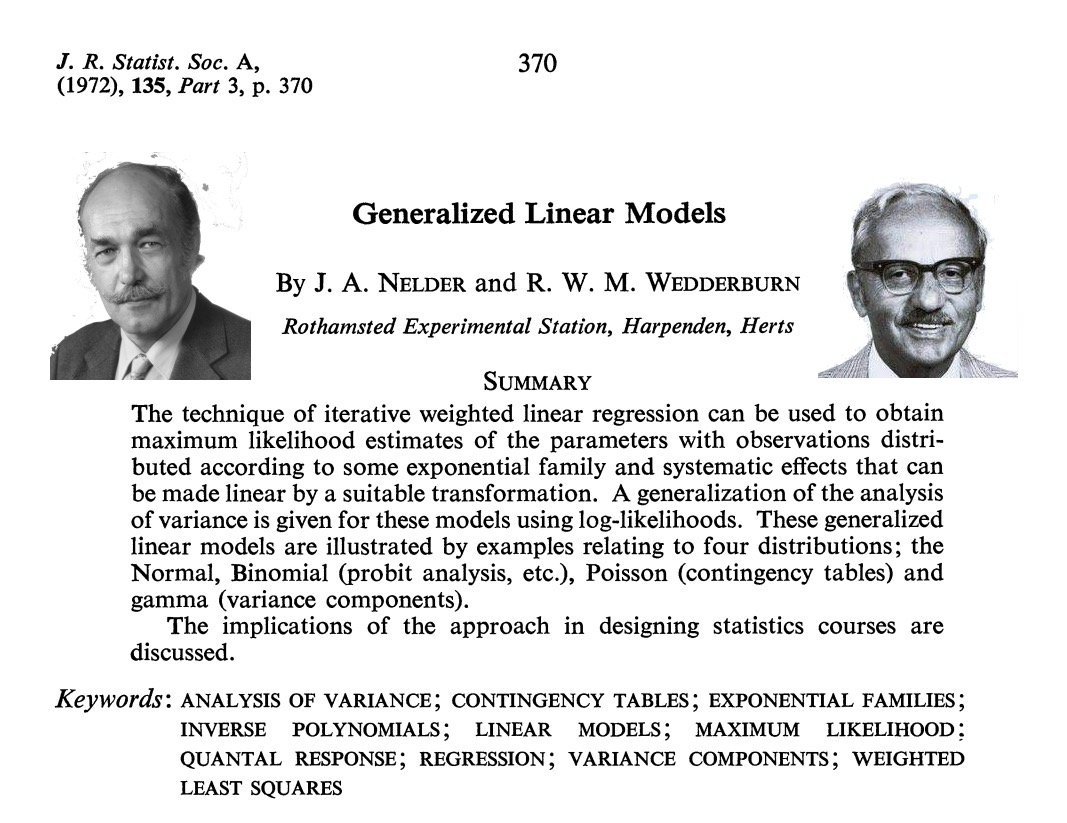
\includegraphics[width=0.9\textwidth, trim={0cm 5cm 0cm 0cm}, clip]{images/glmpub.jpg}
	\end{figure}
\end{frame}

\begin{frame}{Regression Analysis: A brief history}
	\textbf{Generalized Linear Models} \\
	Model assumptions:
	\begin{align*}
		y_i&\stackrel{\hbox{\tiny{ind}}}{\sim} \mathcal{D}(\mu_i,\phi)\\
		\mathbb{E}(y_i)&=\mu_i=h(x_i^\top\beta)
	\end{align*}
	\begin{enumerate}
	\item exponential family response distribution
		\begin{itemize}
			\item normal
			\item Poisson (count regression)
			\item binomial (logistic model)
			\item Gamma
			\item inverse Gaussian
			\item (negative binomial)
		\end{itemize}
	\item constant \textit{dispersion parameter} $\phi$
	\item independence
	\end{enumerate}
\end{frame}

\begin{frame}[c]{Regression Analysis: A brief history}
	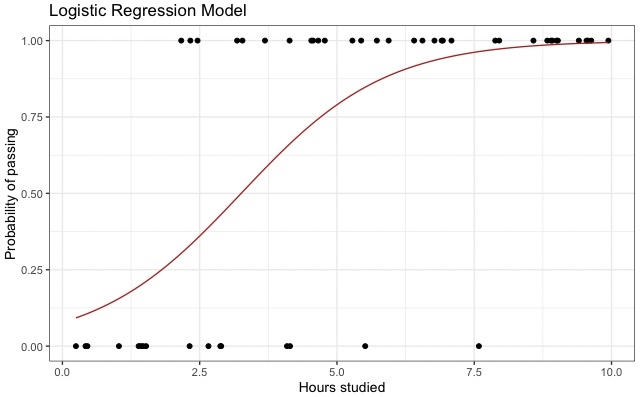
\includegraphics[width=\textwidth]{images/exam_pass_logistic.jpg}
\end{frame}

\begin{frame}{Regression Analysis: A brief history}
	\textbf{Linearity Assumption} \\
	What if our explanatory variables $x_i$ don't have a linear connection with $E(y)$?
	\begin{figure}
		\centering
		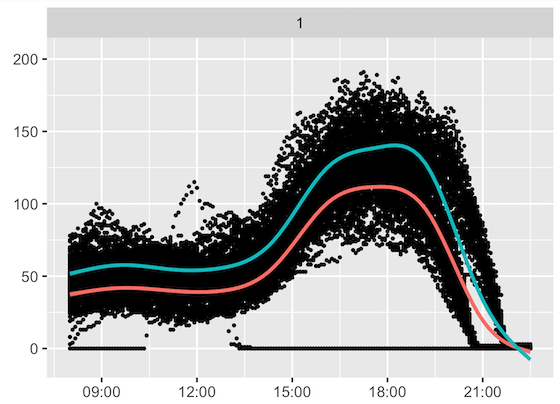
\includegraphics[width=0.85\textwidth, clip, trim = {0cm 0cm 0cm 0.5cm}]{images/nonlinearity.png}
	\end{figure}
\end{frame}

\begin{frame}{Regression Analysis: A brief history}
	\textbf{Generalized Additive Models} \\
	\citet{tibshirani1986}
	\begin{align*}
		y_i&\stackrel{\hbox{\tiny{ind}}}{\sim} \mathcal{E}(\mu_i,\phi)\\
		g(\mu_i)&=\eta_i= s_1(x_{i1})+\ldots+s_J(x_{iJ})
		\end{align*}
		\begin{itemize}
		\item $s_j(x_{ij})$ are parametric \textit{or} smooth functions
		\item Smooth splines can be parametric or non-parametric (penalized)
		\item The $s_j(\cdot)$ can be
			\begin{itemize}
				\item curves (e.g. growth curves)
				\item spatial effects 
				\item varying coefficient terms
				\item interaction surfaces of two continuous variables
				\item random effects
			\end{itemize}
		\end{itemize}
\end{frame}

%---------------------- Section: Distributional Regression --------------------%
\section{Distributional Regression}

\begin{frame}{Distributional Regression}
	\textbf{Back to basics} \\
	What are the three properties (moments) of a distribution?
	\begin{figure}
		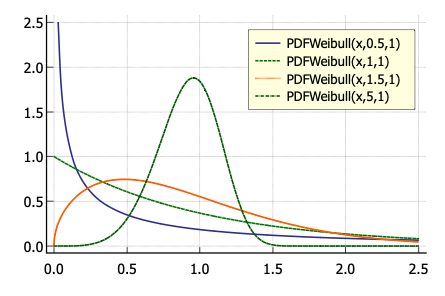
\includegraphics[width = 0.8\textwidth]{images/weibull_all.png}
	\end{figure}
\end{frame}

\begin{frame}{Distributional Regression}
	\textbf{Three properties}
	\begin{itemize}
		\item Location
	\end{itemize}
	\begin{figure}
		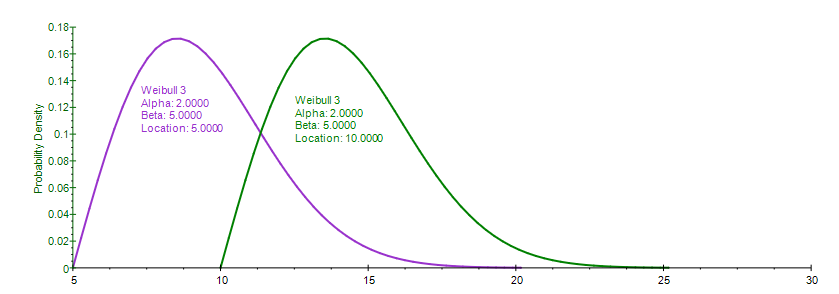
\includegraphics[width=\textwidth]{images/weibull.png}
	\end{figure}
\end{frame}

\begin{frame}{Distributional Regression}
	\textbf{Three properties} \\
	\begin{itemize}
		\item Scale
	\end{itemize}
	\begin{figure}
		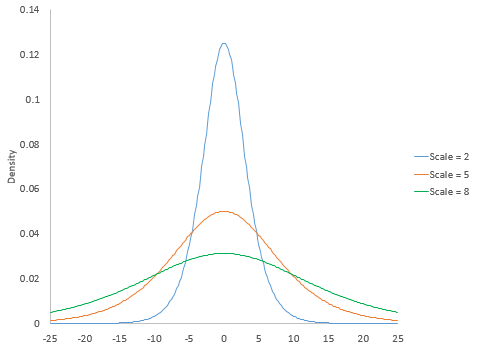
\includegraphics[width=0.8\textwidth]{images/scale.png}
	\end{figure}
\end{frame}

\begin{frame}{Distributional Regression}
	\textbf{Three properties} \\
	\citet{chartio_histogram}
	\begin{itemize}
		\item Shape
	\end{itemize}
	\begin{figure}
		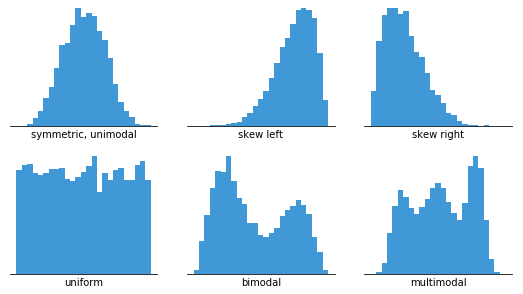
\includegraphics[width=\textwidth]{images/histogram-example-2}
	\end{figure}
\end{frame}

\begin{frame}{Distributional Regression}
	``It is difficult to understand why statisticians commonly limit their enquiries to
Averages, and do not revel in more comprehensive views. Their souls seem as dull to
the charm of variety as that of the native of one of our flat English counties, whose retrospect of Switzerland was that, if its mountains could be thrown into its lakes, two nuisances would be got rid of at once.'' \\
- Sir Francis Galton (England, 1822-1911)
\begin{figure}
	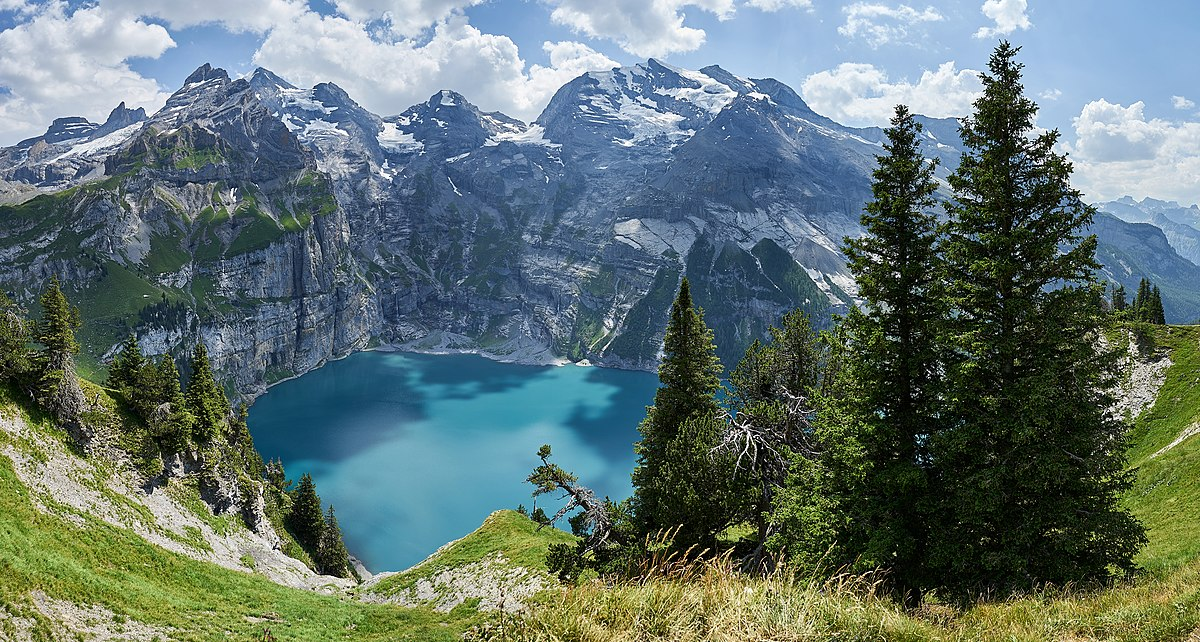
\includegraphics[width=0.75\textwidth]{images/oeschinensee.jpg}
\end{figure}
\end{frame}

\begin{frame}{Distributional Regression}
	\textbf{An expected result} \\
	``...most empirical modelling is firmly located in the lowlands of the conditional expectation of the distribution of the response, e.g. in generalized linear models.'' \\ 
	\citep{rage_mean}
	\begin{itemize}
		\item Linear Models, GLM, GAM centered around finding the mean of a distribution
		\item What about all the other properties?
	\end{itemize}
\end{frame}

% \begin{frame}{Distributional Regression}
% 	\begin{figure}
% 		\centering
% 		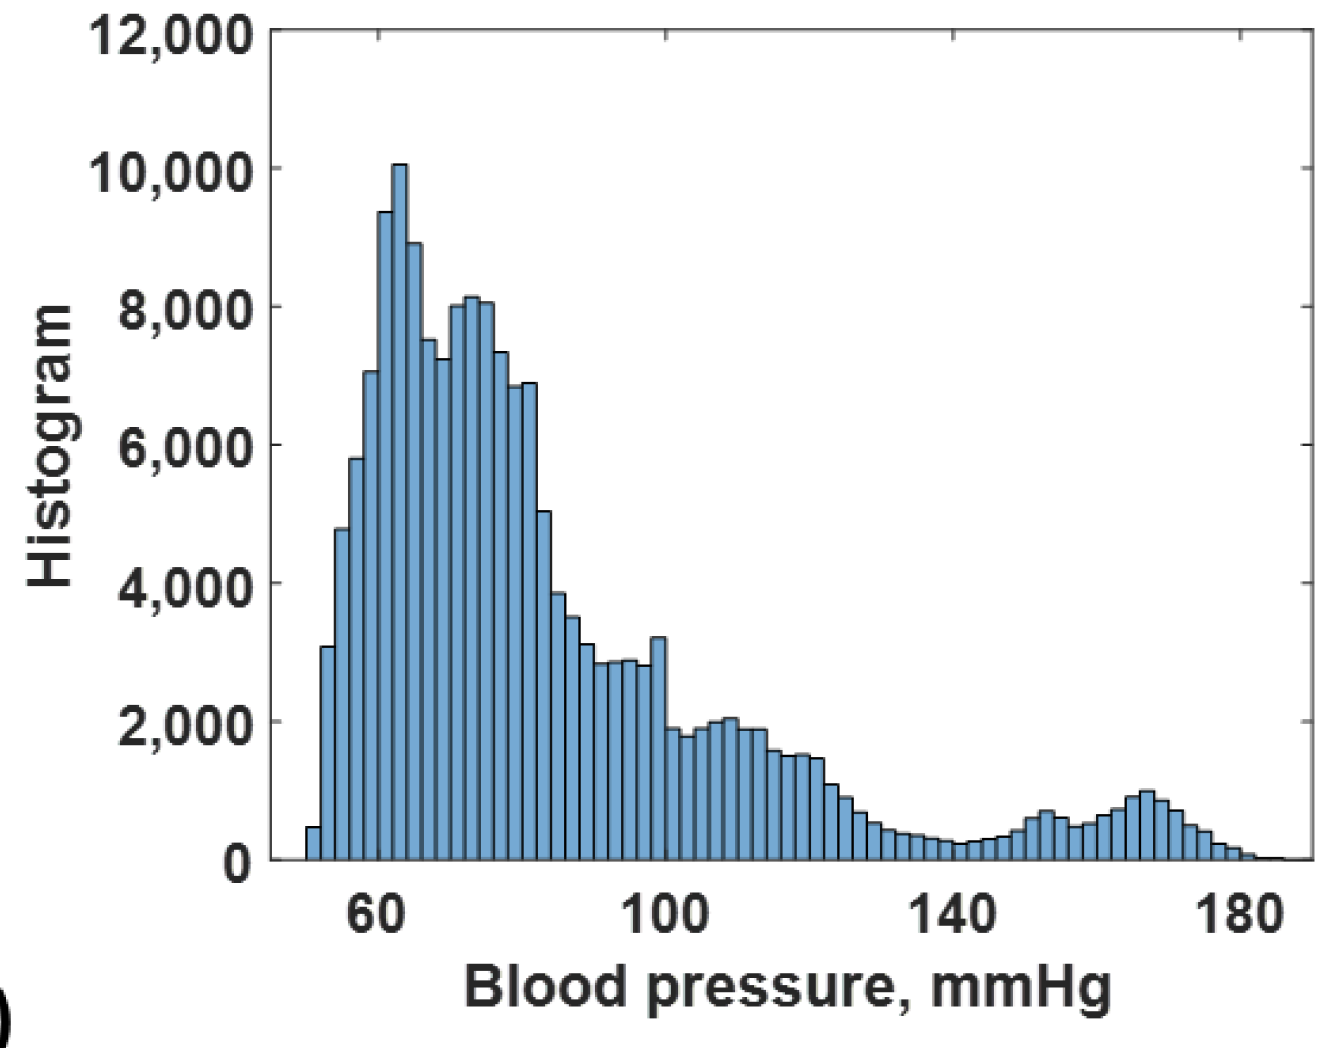
\includegraphics[width=0.8\textwidth, clip, trim = {0.2cm 0cm 0cm 0cm}]{images/blood_pressure.png}
% 	\end{figure}
% 	\citep*{bloodpressure}
% \end{frame}

% \begin{frame}{Distributional Regression}
% 	blood pressure variability effect on risk of cardiovascular disease
% 	https://www.bmj.com/content/354/bmj.i4098
% \end{frame}

\begin{frame}{Distributional Regression}
	\textbf{An example} \\
	\begin{figure}
		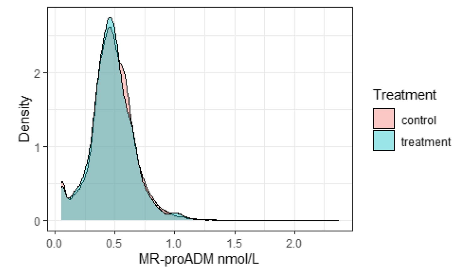
\includegraphics[width=0.8\textwidth]{images/mr_proadm_dist.png}
		\caption{Kernel Density estimate of MR-proADM (a biomarker used on coronary heart disease), as seen in \citet{heller2022}}
	\end{figure}
	\begin{itemize}
		\item Does \textit{Pravastatin} change the distribution of \textit{MR-proADM}?
	\end{itemize}
\end{frame}

\begin{frame}{Distributional Regression}
	\textbf{MR-proADM biomarker} \\
	\begin{itemize}
		\item Four scenarios:
		\begin{enumerate}
			\item Normal (reduced)
			\item BCT (reduced)
			\item Normal (extended)
			\item BCT (extended)
		\end{enumerate}
	\end{itemize}
	\pause
	\begin{figure}
		\centering
		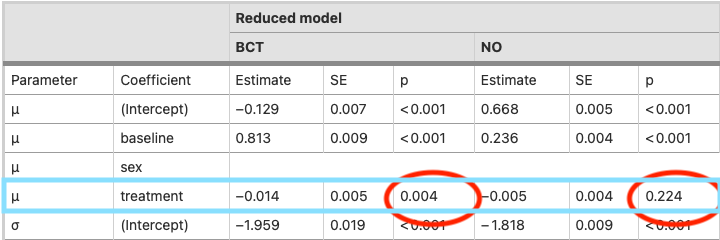
\includegraphics[width=\textwidth]{images/gillian_table1.png}
	\end{figure}
	Treatment effect. Is that it?
\end{frame}

\begin{frame}{Distributional Regression}
	\textbf{MR-proADM biomarker} \\
	Scenario 3 \& 4 (extended)
	\begin{figure}
		\centering
		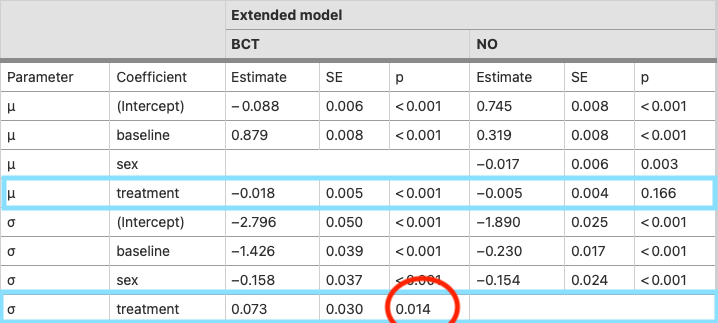
\includegraphics[width=\textwidth]{images/gillian_table2.png}
	\end{figure}
	\begin{itemize}
		\item Treatment effect on the scale parameter
		\item From unsuccessful to successful
	\end{itemize}
\end{frame}

\begin{frame}{Distributional Regression}
	\textbf{Overview} \\
	Let $y \sim D(\alpha_1, \ldots, \alpha_K)$. With distributional regression...
	\begin{itemize}
	  \item Every parameter $\alpha_i$ can be modeled using a (different) set of predictors
	  \item Predictors can take different forms, e.g. non-linear, spatial, random effects
	  \item Parameters are connected to the predictors using link-functions that uphold the support of the parameter
	\end{itemize}
	\textbf{Model Equations} \\
	$\Rightarrow$ This allows for extremely flexible model equations:
	\begin{equation}
	g_l(\boldsymbol{\alpha}_l) = f_{1l}(\mathbf{X}_{1l} ; \boldsymbol{\theta}_{1l}) + \ldots + f_{Q_{l}l}(\mathbf{X}_{Q_ll} ; \boldsymbol{\theta}_{Q_{l}l})
	\end{equation}
\end{frame}

\begin{frame}{Distributional Regression}
	\textbf{Precipitation in Austria} \\
	\citet{bamlss2017}
	\begin{figure}
		\centering
		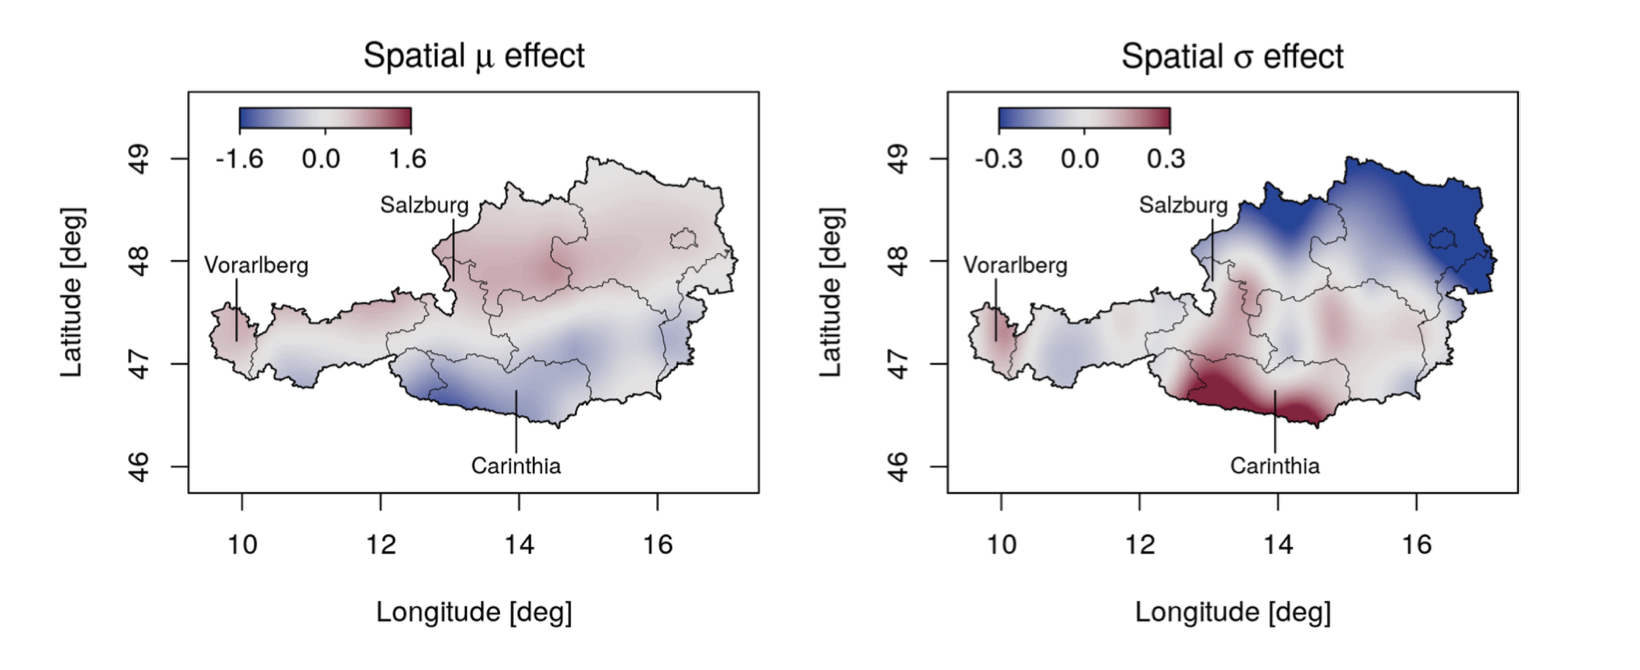
\includegraphics[width=1.1\textwidth]{images/precipitation_austria.png}
	\end{figure}
	\begin{itemize}
		\item Mean and variance spatial effect on precipitation
	\end{itemize}
\end{frame}

\begin{frame}{Distributional Regression}
	\textbf{In Practice} \\
	Implementations in R:
	\begin{itemize}
		\item gamlss \citep[Generalized Additive Models for Location, Scale and Shape]{gamlssbook}
		\item bamlss \citep{bamlss2017}
		\item VGAM \citep[Vector Generalized Additive Models]{vgampackage}
	\end{itemize}
	\begin{figure}
		\centering
		
\includegraphics[scale=0.5, trim={0cm 0.2cm 0cm 0cm}, clip]{images/gamlss_logo.png}
	\end{figure}
\end{frame}

\begin{frame}{Distributional Regression}
	\textbf{How to get started} \\
	\begin{figure}
		\centering
		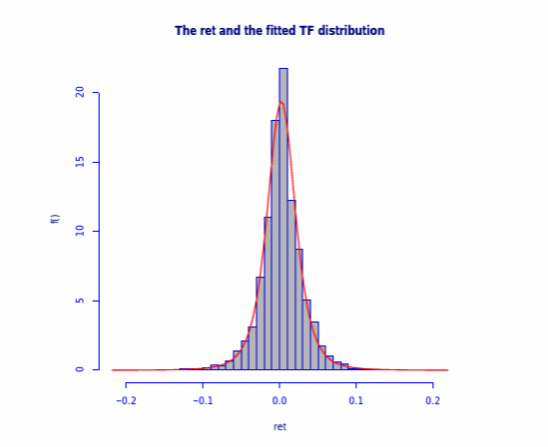
\includegraphics[width=0.7\textwidth]{images/turkish_stock.png}
		\caption{Turkish stock exchange returns, taken from \citet{gamlssbook}}
	\end{figure}
\end{frame}

\begin{frame}{Distributional Regression}
	\textbf{How to get started} \\
	\begin{itemize}
		\item \texttt{fitDist()} function can select the right distribution for your data
		\item Conditional distributions (as dependent on your data) can be fitted as well
	\end{itemize}
	\begin{figure}
		\centering
		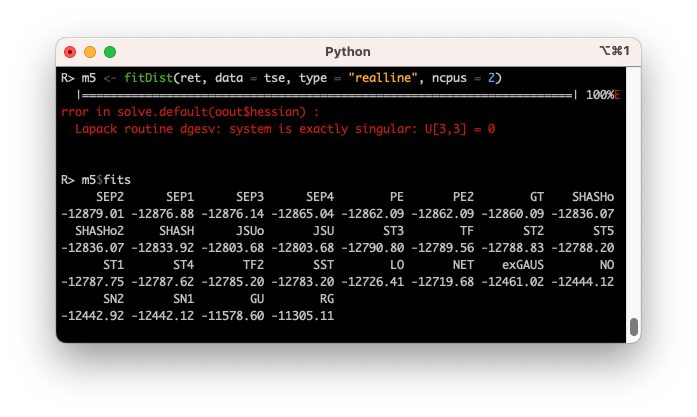
\includegraphics[width=\textwidth]{images/fitdist_gamlss.png}
	\end{figure}
\end{frame}

\begin{frame}{Distributional Regression}
	\textbf{How to get started} \\
	\begin{itemize}
		\item \texttt{fitDist()} function can select the right distribution for your data
		\item Conditional distributions (as dependent on your data) can be fitted as well
	\end{itemize}
	\begin{figure}
		\centering
		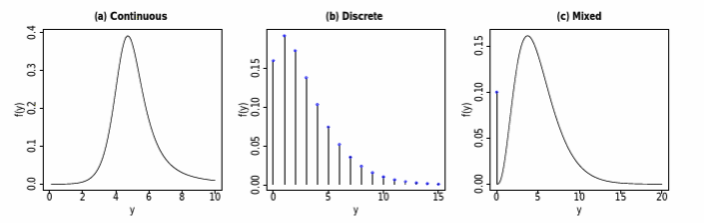
\includegraphics[width=\textwidth]{images/gamlss_dists.png}
	\end{figure}
\end{frame}

\begin{frame}{Distributional Regression}
	\textbf{How to get started} \\
	Once you are ready to fit your model...
	\begin{figure}
		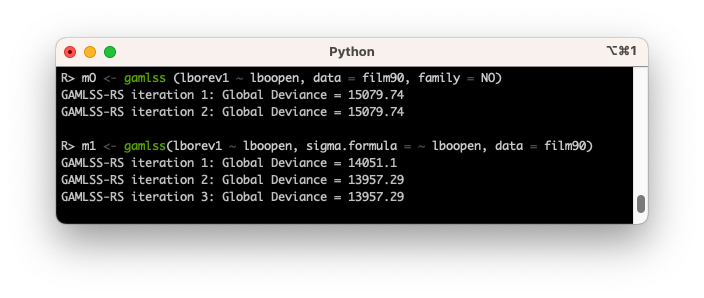
\includegraphics[width=\textwidth]{images/code_gamlss1.png}
	\end{figure}
	\begin{itemize}
		\item $\mu$ term fitted just as in normal linear regression
		\item \texttt{sigma.formula} argument for $\sigma$
	\end{itemize}
\end{frame}

\begin{frame}{Distributional Regression}
	\textbf{How to get started}
	\vspace{-0.3cm}
	\begin{figure}
		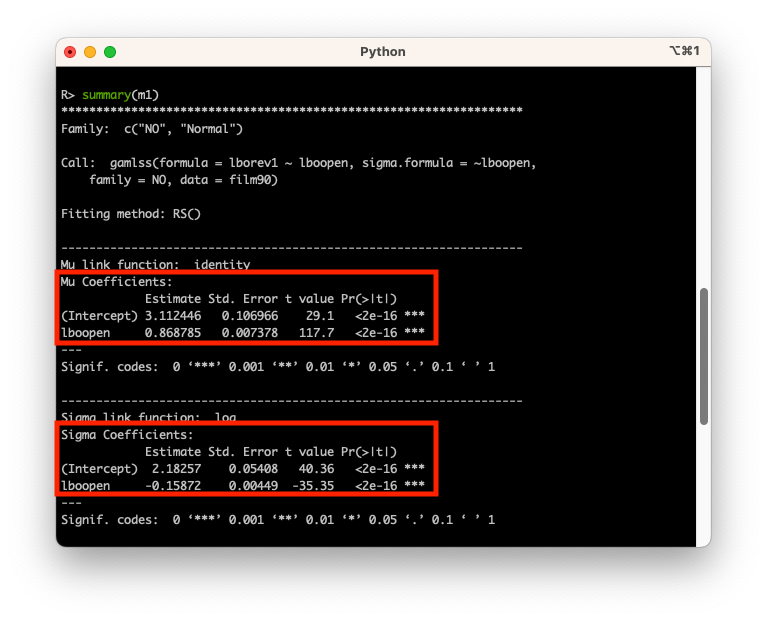
\includegraphics[width=\textwidth]{images/code_gamlss2.png}
	\end{figure}
\end{frame}

\begin{frame}{Distributional Regression}
	\textbf{Post-model diagnostics} \\
	\citet{stadlmann2022}: \texttt{distreg.vis}
	\begin{figure}
		\centering
		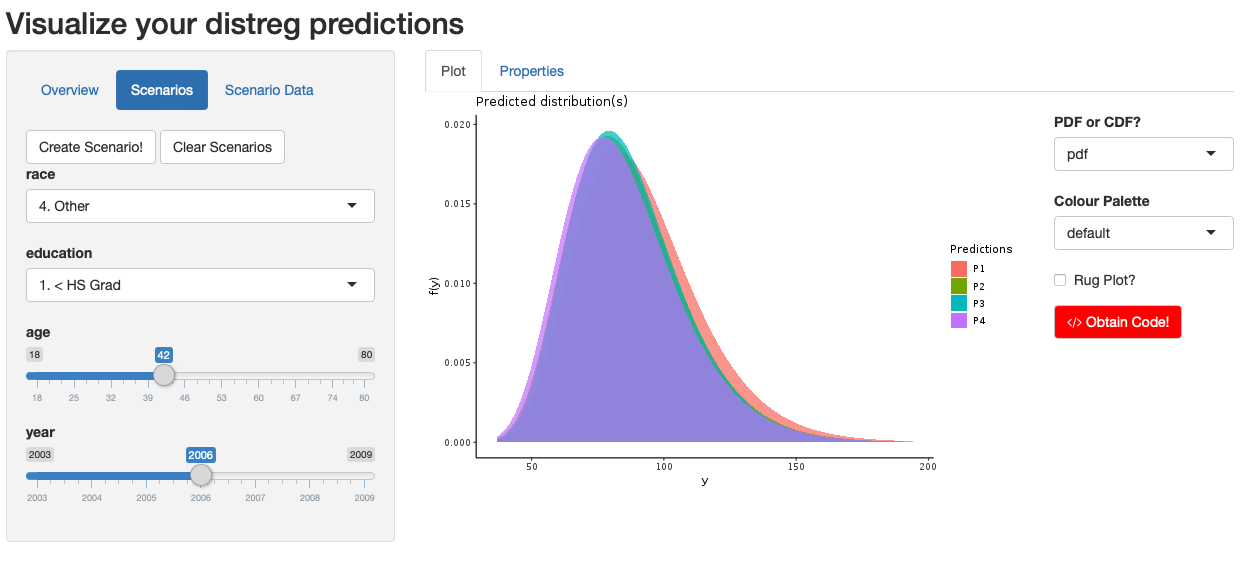
\includegraphics[width=\textwidth]{images/distreg.vis.png}
	\end{figure}
\end{frame}

\begin{frame}[c]{Thank you}
	\centering
	Thank you! \\
	
\includegraphics[width=0.8\textwidth]{images/URL.png}
\end{frame}

\begin{frame}[c]{Thank you}
	\centering
	Questions? \\
	
\includegraphics[width=0.8\textwidth]{images/URL.png}
\end{frame}

\section*{References}

\AtBeginSection{}

\begin{frame}[allowframebreaks]
	\bibliography{98_references}
	\bibliographystyle{apacite}
\end{frame}

\end{document}


%%% Local Variables:
%%% mode: latex
%%% TeX-master: t
%%% End:
